\section{FESDModelv2 Results}

The results of the testing after 50 epochs of training for FESDModelv2 can be seen in table \ref{tab:res_v2}. The numeric values of the accuracy and F1-Score are within a good range. However, the percentage of positive guesses metric indicates that the model is overfitting and only predicts positive values.

\begin{table}[!htbp]
  \caption[Test Results of FESDModelv1]{The test results of FESDModelv1 after 50 epochs of training.}
  \label{tab:res_v1}
  \begin{tabular}{lrrrrr}
    \hline
    {} &  Percentage of positive guesses &  Accuracy &  F1-Score &  F2-Score &  Cohen's Kappa Coefficient \\
    Problem Set   &                                 &           &           &           &                            \\
    \hline
    Full Body  &                          50.417 &     0.688 &     0.458 &     0.673 &                      0.397 \\
    Half Body  &                          55.833 &     0.767 &     0.446 &     0.789 &                      0.554 \\
    Body Parts &                          79.028 &     0.779 &     0.722 &     0.842 &                      0.257 \\
    Joints     &                          70.000 &     0.892 &     0.638 &     0.918 &                      0.773 \\
    \hline
  \end{tabular}
\end{table}

The results shown in table \ref{tab:res_v2} are reflected in the confusion matrices seen in figure \ref{fig:conf_v2}. The half-body and body parts problem set only guess positive results, hence the Percentage of positive guesses. The Cohen's Kappa Coefficient is 0 if $tp \cdot tn = fn \cdot fp$. This is the case if only one class is guessed, which is the case if all guesses are positive.

The ROC curves shown in figure \ref{fig:roc_v2}, show the different true positive and false positive rates for each of the areas in each problem set.

The results of the model developed to detect errors in the Joint Problem set are in a good range when considering all joints together. However, when considering the confusion matrix for each of the joints, as can be seen in figure \ref{fig:conf_v2_jts}, the show that while in total not a single error label is guessed all the time for all joints together, each joint does not have varying error labels and is therefore not a good model for this dataset. 

Similar to FESDModelv1, the Half Body problem set is producing very good predictions which do not indicate overfitting. In figure \ref{fig:conf_v2_hb_ul} the confusion matrices can be seen for the upper and lower body. It can be seen that the detection of the lower body is more successful than the detection of the upper body. It is important to note, that the upper body has far more stable joints and more joints in general. The difference in accuracy when predicting errors in the lower and upper body is possibly caused by this distribution of stable joints.

\begin{figure}[htbp]
  \centering
  \begin{subfigure}[b]{0.4\linewidth}
      \centering
      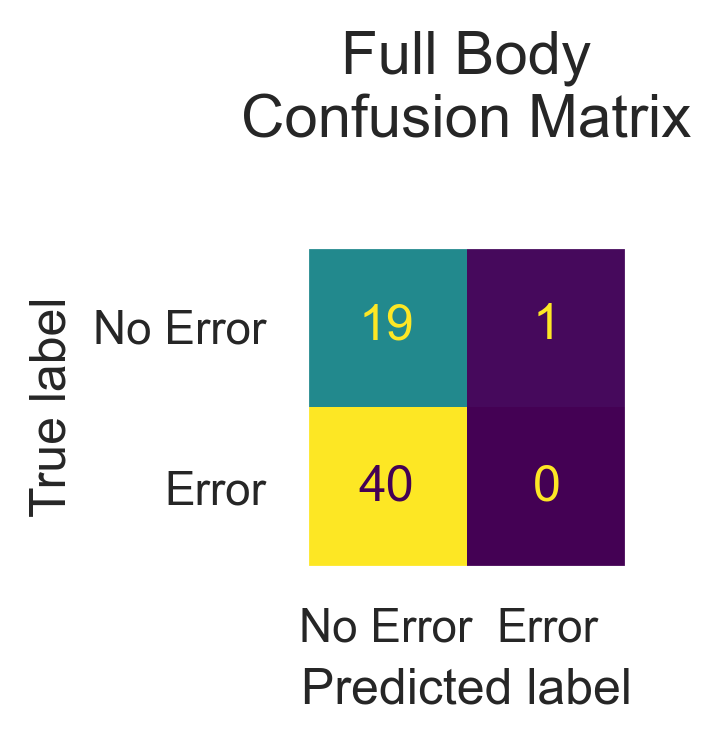
\includegraphics[width=\textwidth]{figures/Results/v2/confusion/full_together.png}
      \caption[]{Full Body Problem Set}
      \label{fig:fb_conf}
  \end{subfigure}
  \hfill
  \begin{subfigure}[b]{0.4\linewidth}
      \centering
      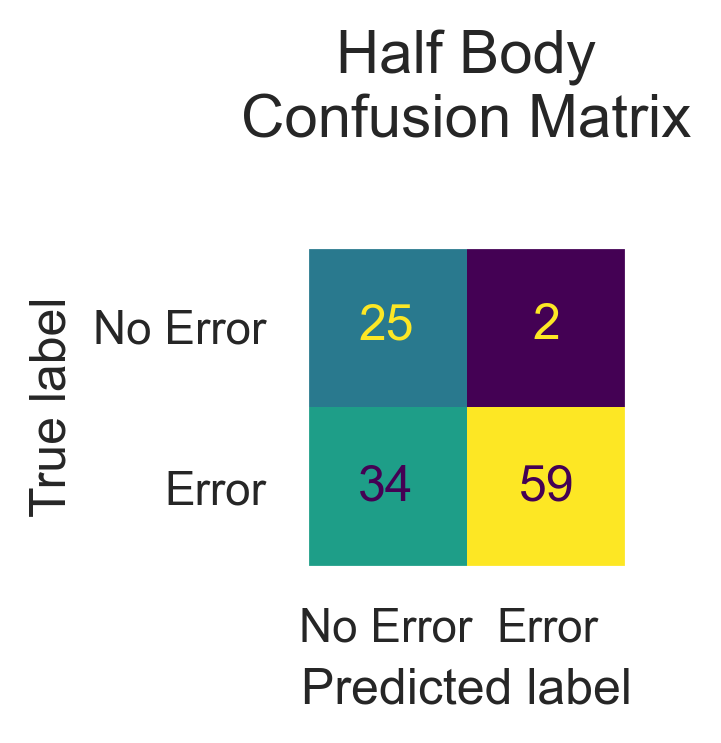
\includegraphics[width=\textwidth]{figures/Results/v2/confusion/half_together.png}
      \caption{Half Body Problem Set}
      \label{fig:hb_conf}
  \end{subfigure}
  \hfill
  \begin{subfigure}[b]{0.4\linewidth}
      \centering
      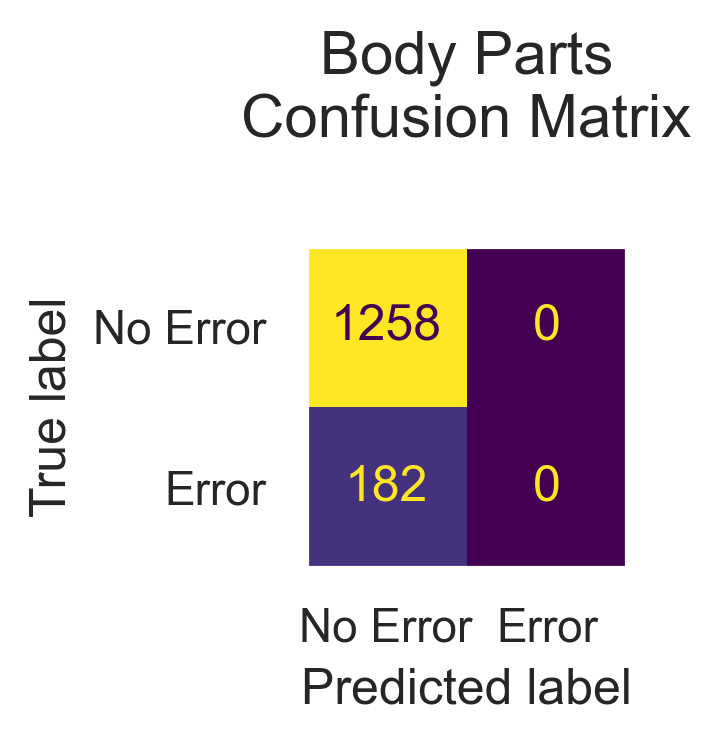
\includegraphics[width=\textwidth]{figures/Results/v2/confusion/body_parts_together.png}
      \caption{Body Part Problem Set}
      \label{fig:bp_conf}
  \end{subfigure}
  \hfill
  \begin{subfigure}[b]{0.4\linewidth}
      \centering
      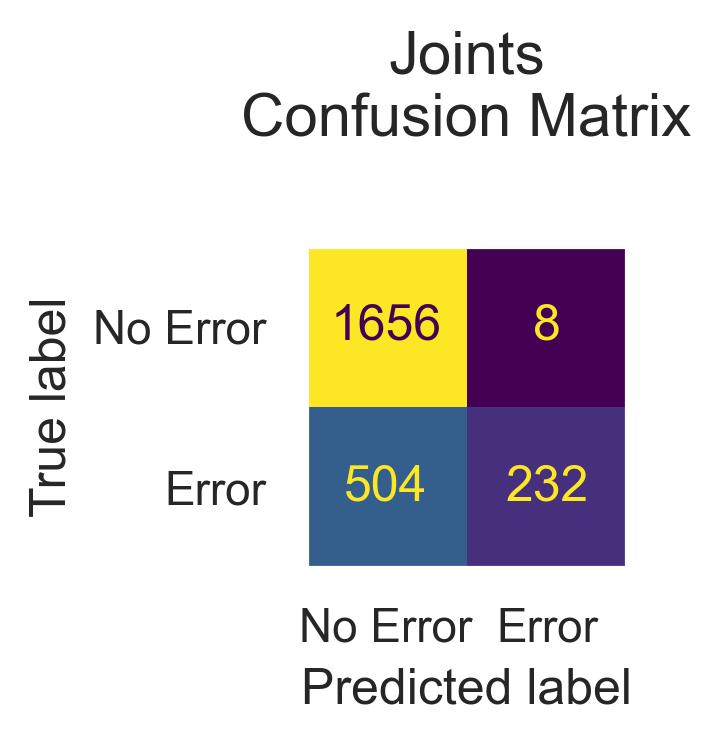
\includegraphics[width=\textwidth]{figures/Results/v2/confusion/joints_together.png}
      \caption{Joint Problem Set}
      \label{fig:jt_conf}
  \end{subfigure}
  \caption[Confusion Matrices of FESDModelv2]{The confusion Matrices of FESDModelv2.}
  \label{fig:conf_v2}
\end{figure}

\begin{figure}[htbp]
  \centering
  \begin{subfigure}[b]{0.4\linewidth}
      \centering
      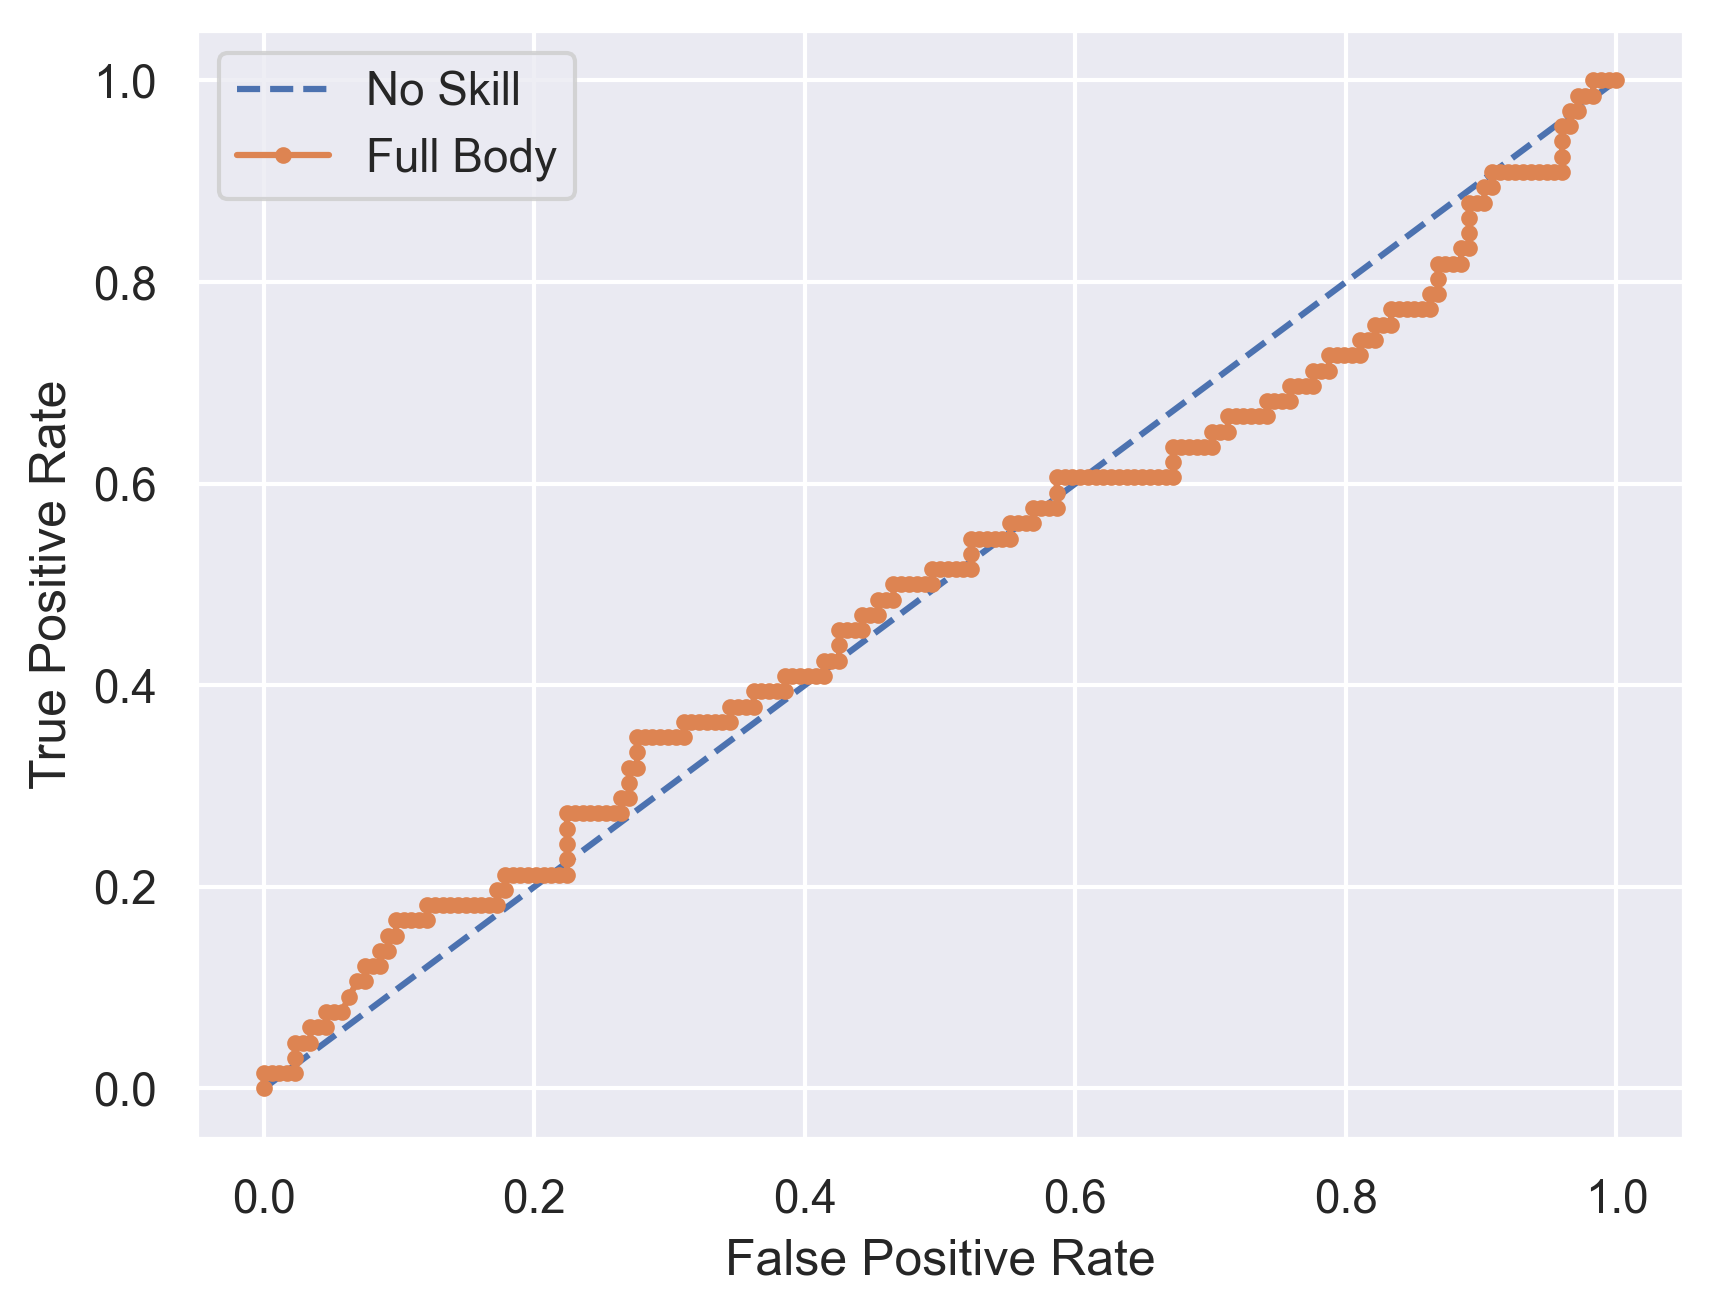
\includegraphics[width=\textwidth]{figures/Results/v2/roc/fb.png}
      \caption[]{Full Body Problem Set}
      \label{fig:fb_roc_v2}
  \end{subfigure}
  \hfill
  \begin{subfigure}[b]{0.4\linewidth}
      \centering
      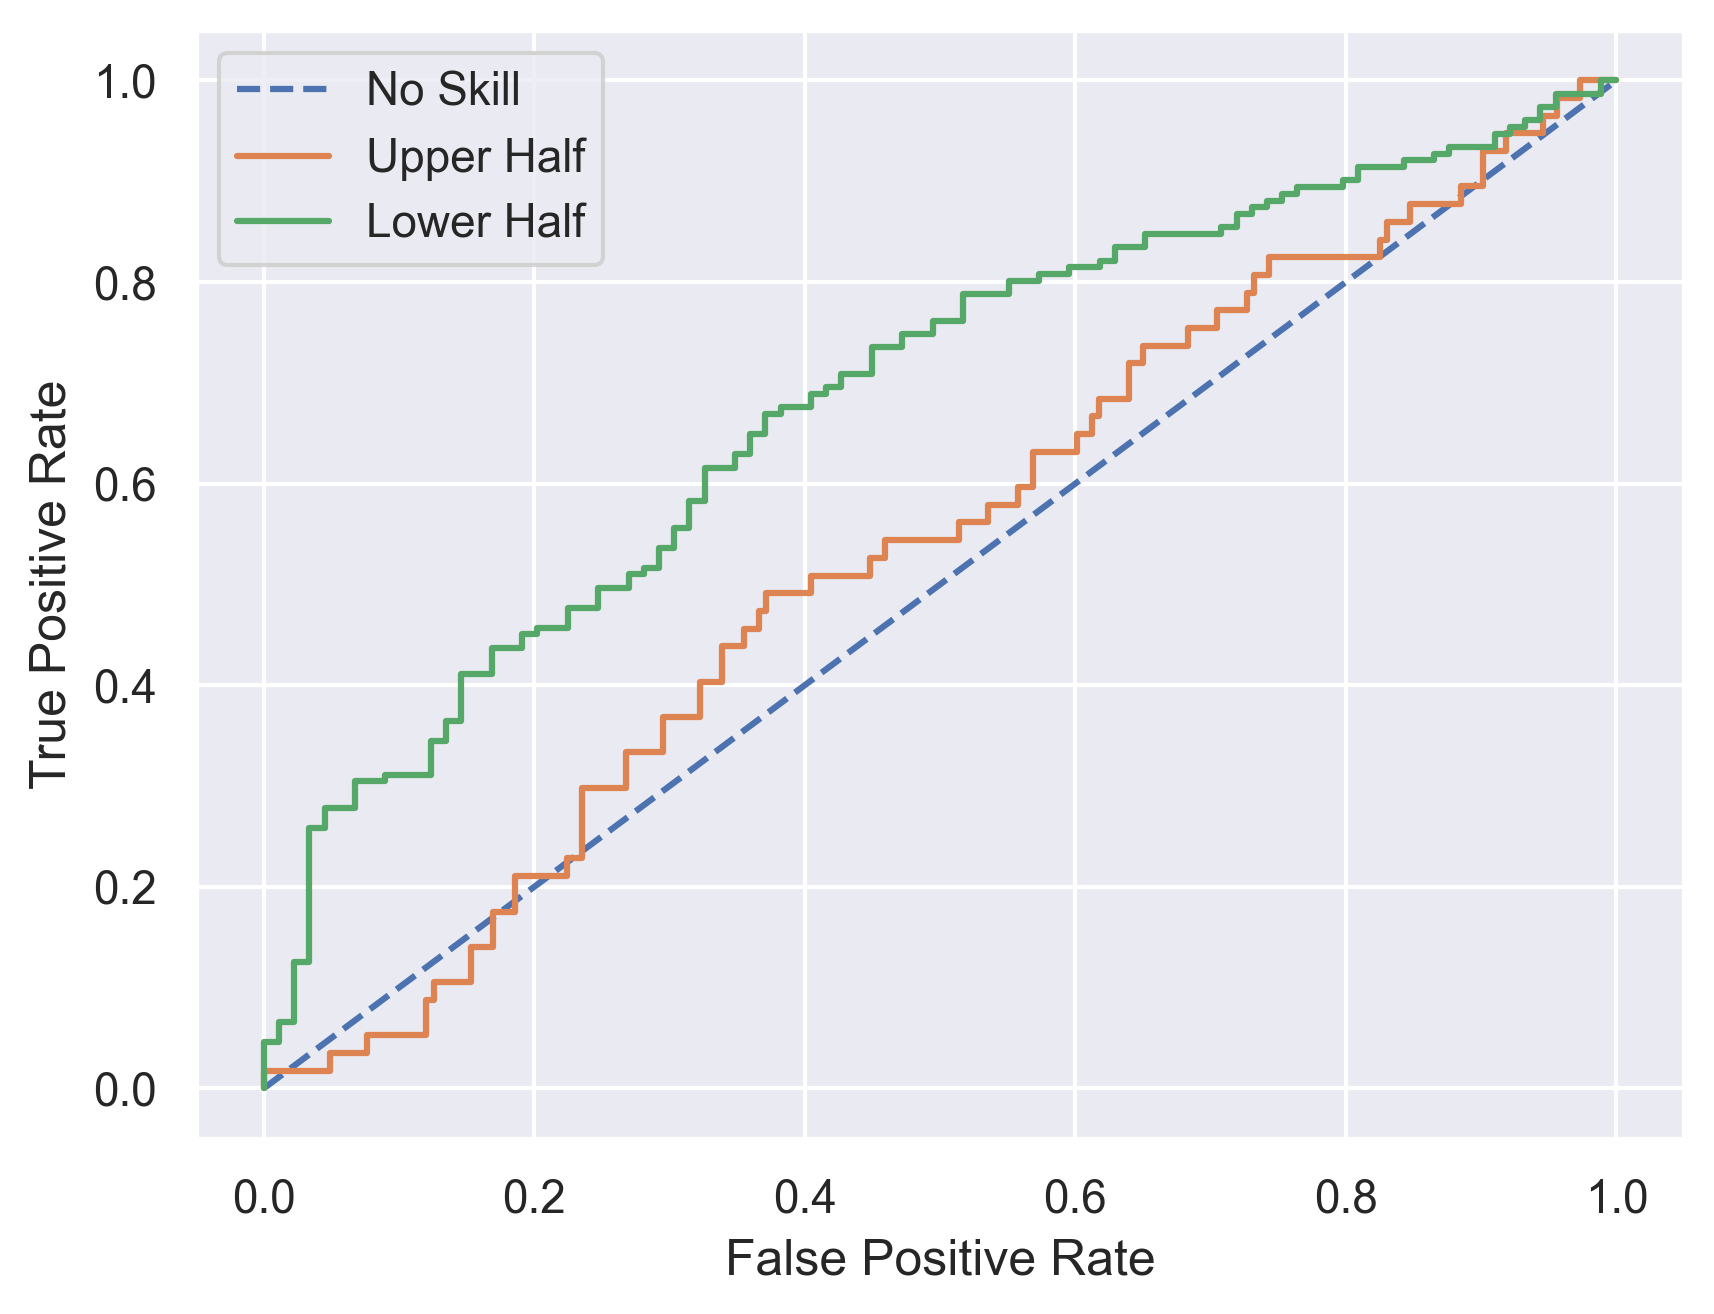
\includegraphics[width=\textwidth]{figures/Results/v2/roc/hb.png}
      \caption[]{Half Body Problem Set}
      \label{fig:hb_roc_v2}
  \end{subfigure}
  \hfill
  \begin{subfigure}[b]{0.4\linewidth}
      \centering
      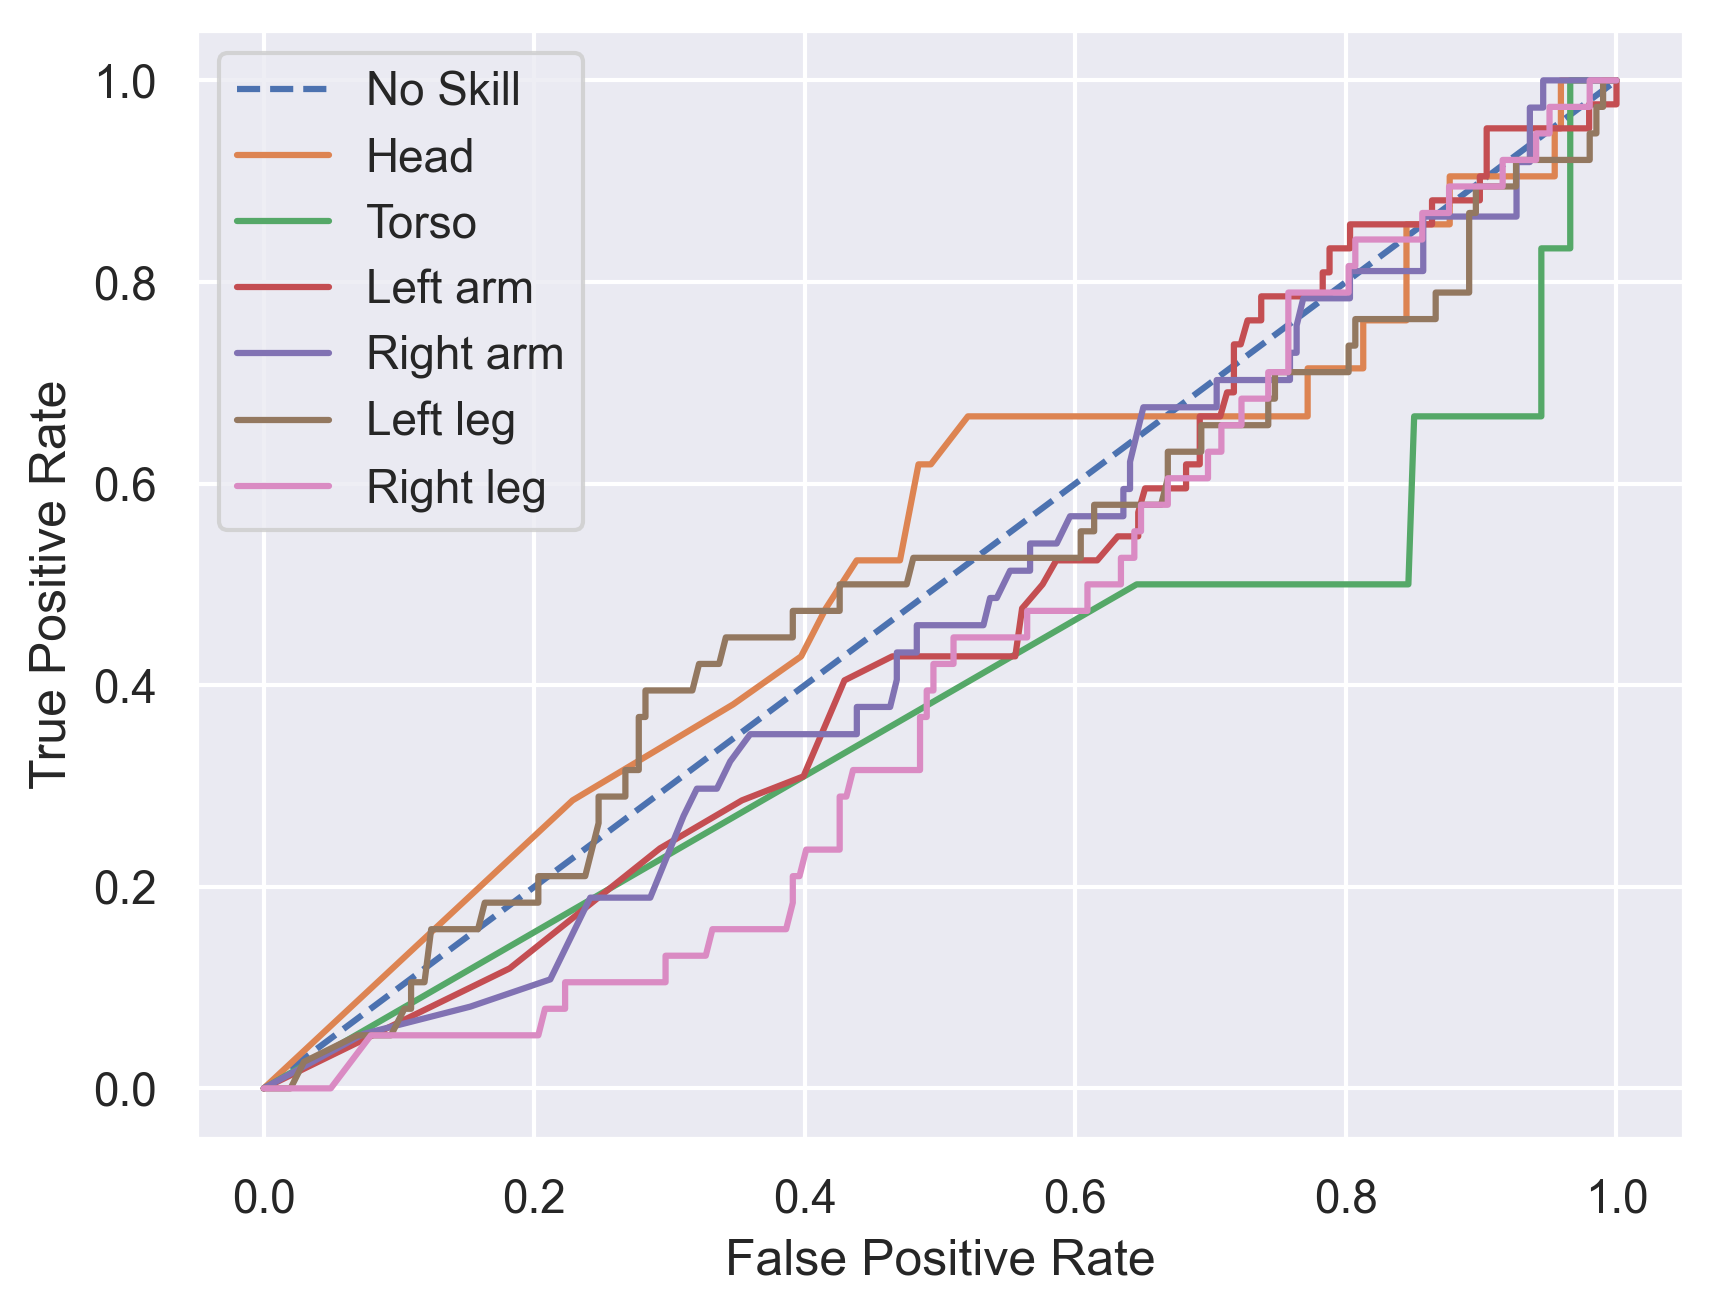
\includegraphics[width=\textwidth]{figures/Results/v2/roc/bp.png}
      \caption[]{Body Part Problem Set}
      \label{fig:bp_roc_v2}
  \end{subfigure}
  \hfill
  \begin{subfigure}[b]{0.4\linewidth}
      \centering
      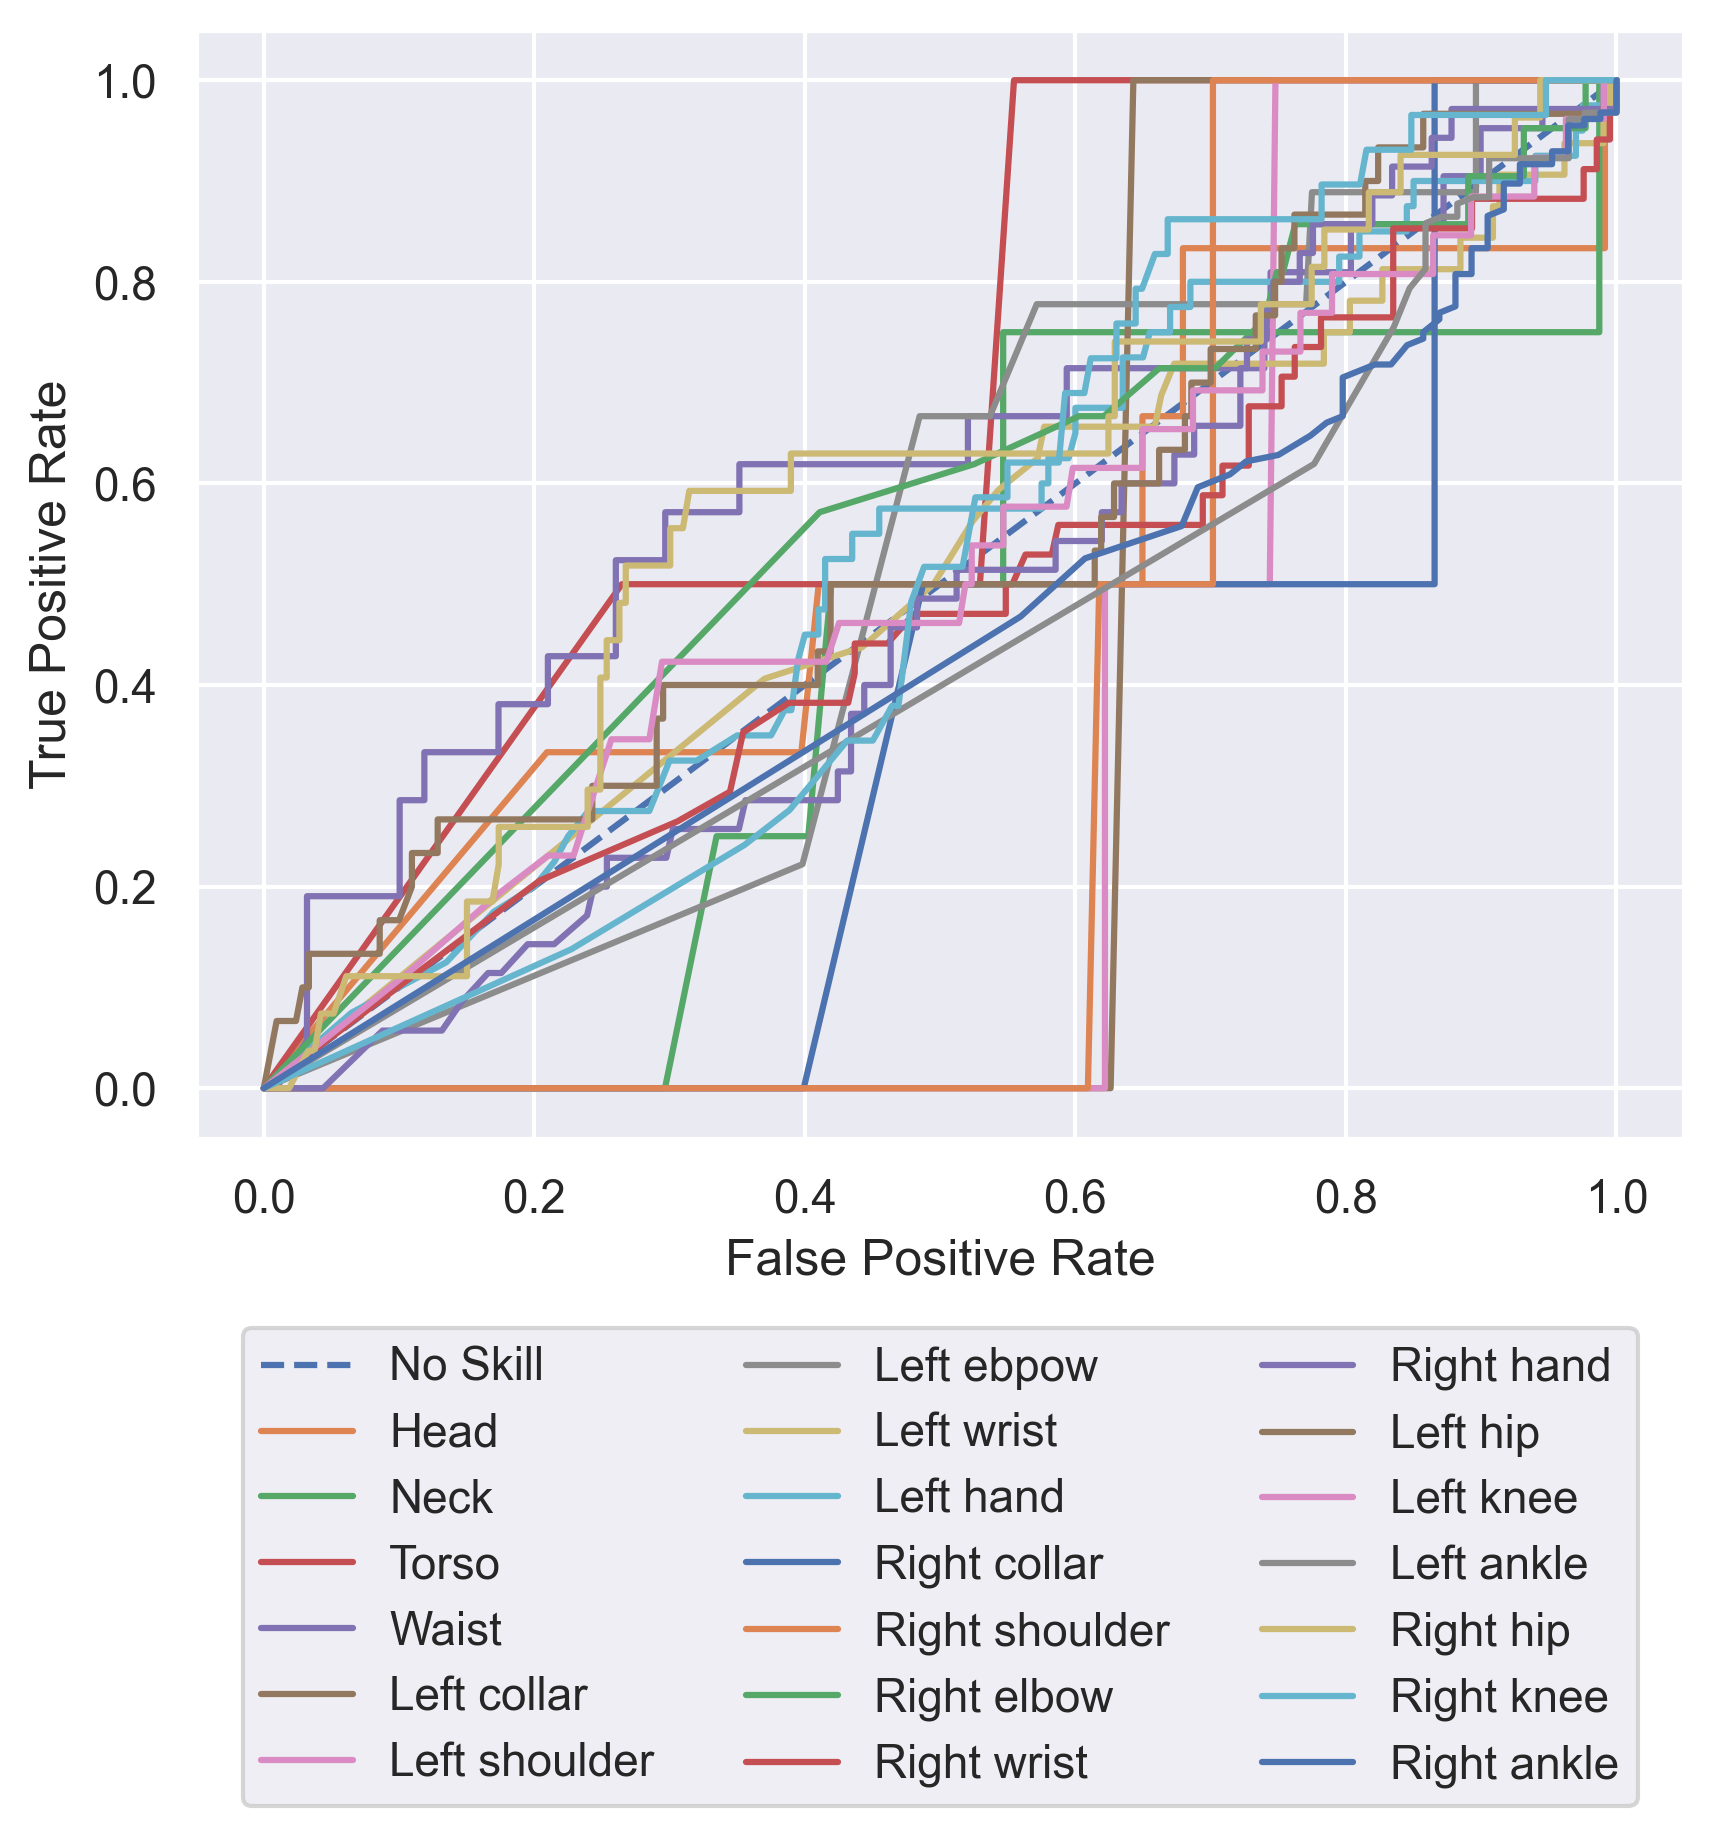
\includegraphics[width=\textwidth]{figures/Results/v2/roc/jt.png}
      \caption[]{Joint Problem Set}
      \label{fig:jt_roc_v2}
  \end{subfigure}
  \caption[ROC Curves of FESDModelv2]{The ROC curves of FESDModelv2.}
  \label{fig:roc_v2}
\end{figure}

\begin{figure}[htbp]
  \centering
  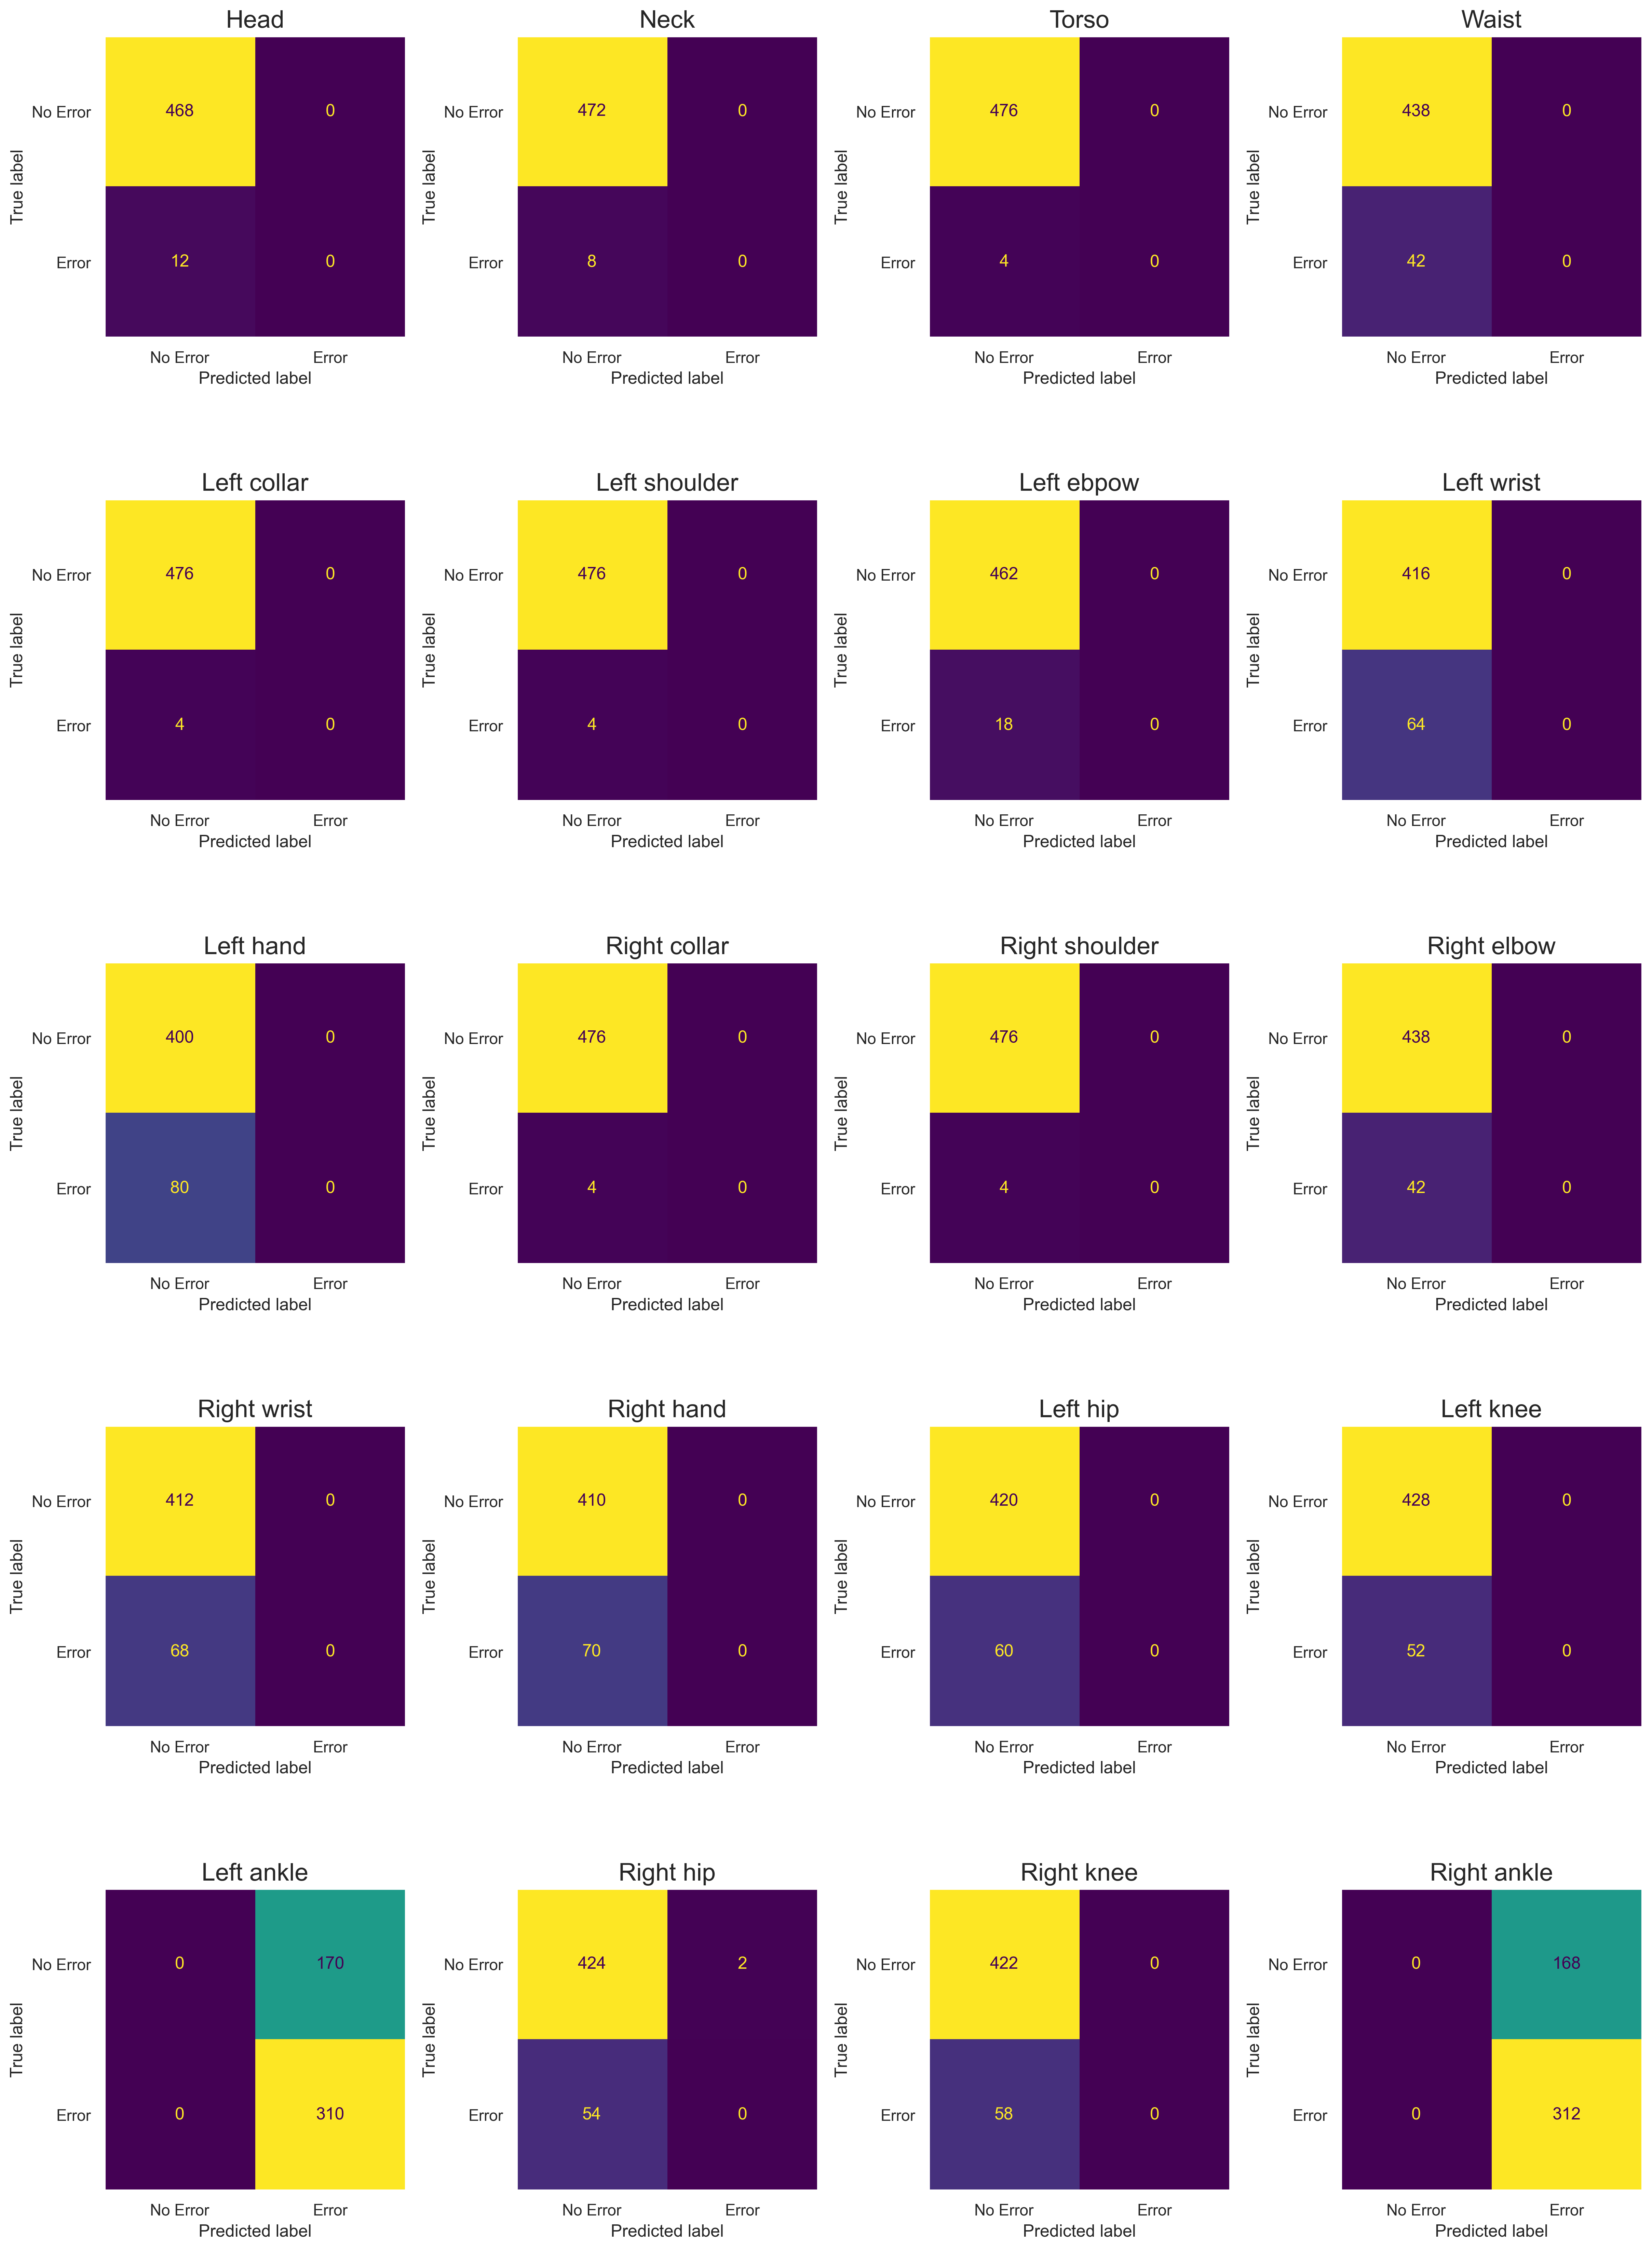
\includegraphics[width=.8\linewidth]{figures/Results/v2/confusion/joints_joint.png}
  \caption[Confusion matrix of FESDModelv2 for each Joint]{The confusion matrix of each joint for FESDModelv2 for the joint problem set.}
  \label{fig:conf_v2_jts}
\end{figure}

\begin{figure}[htbp]
  \centering
  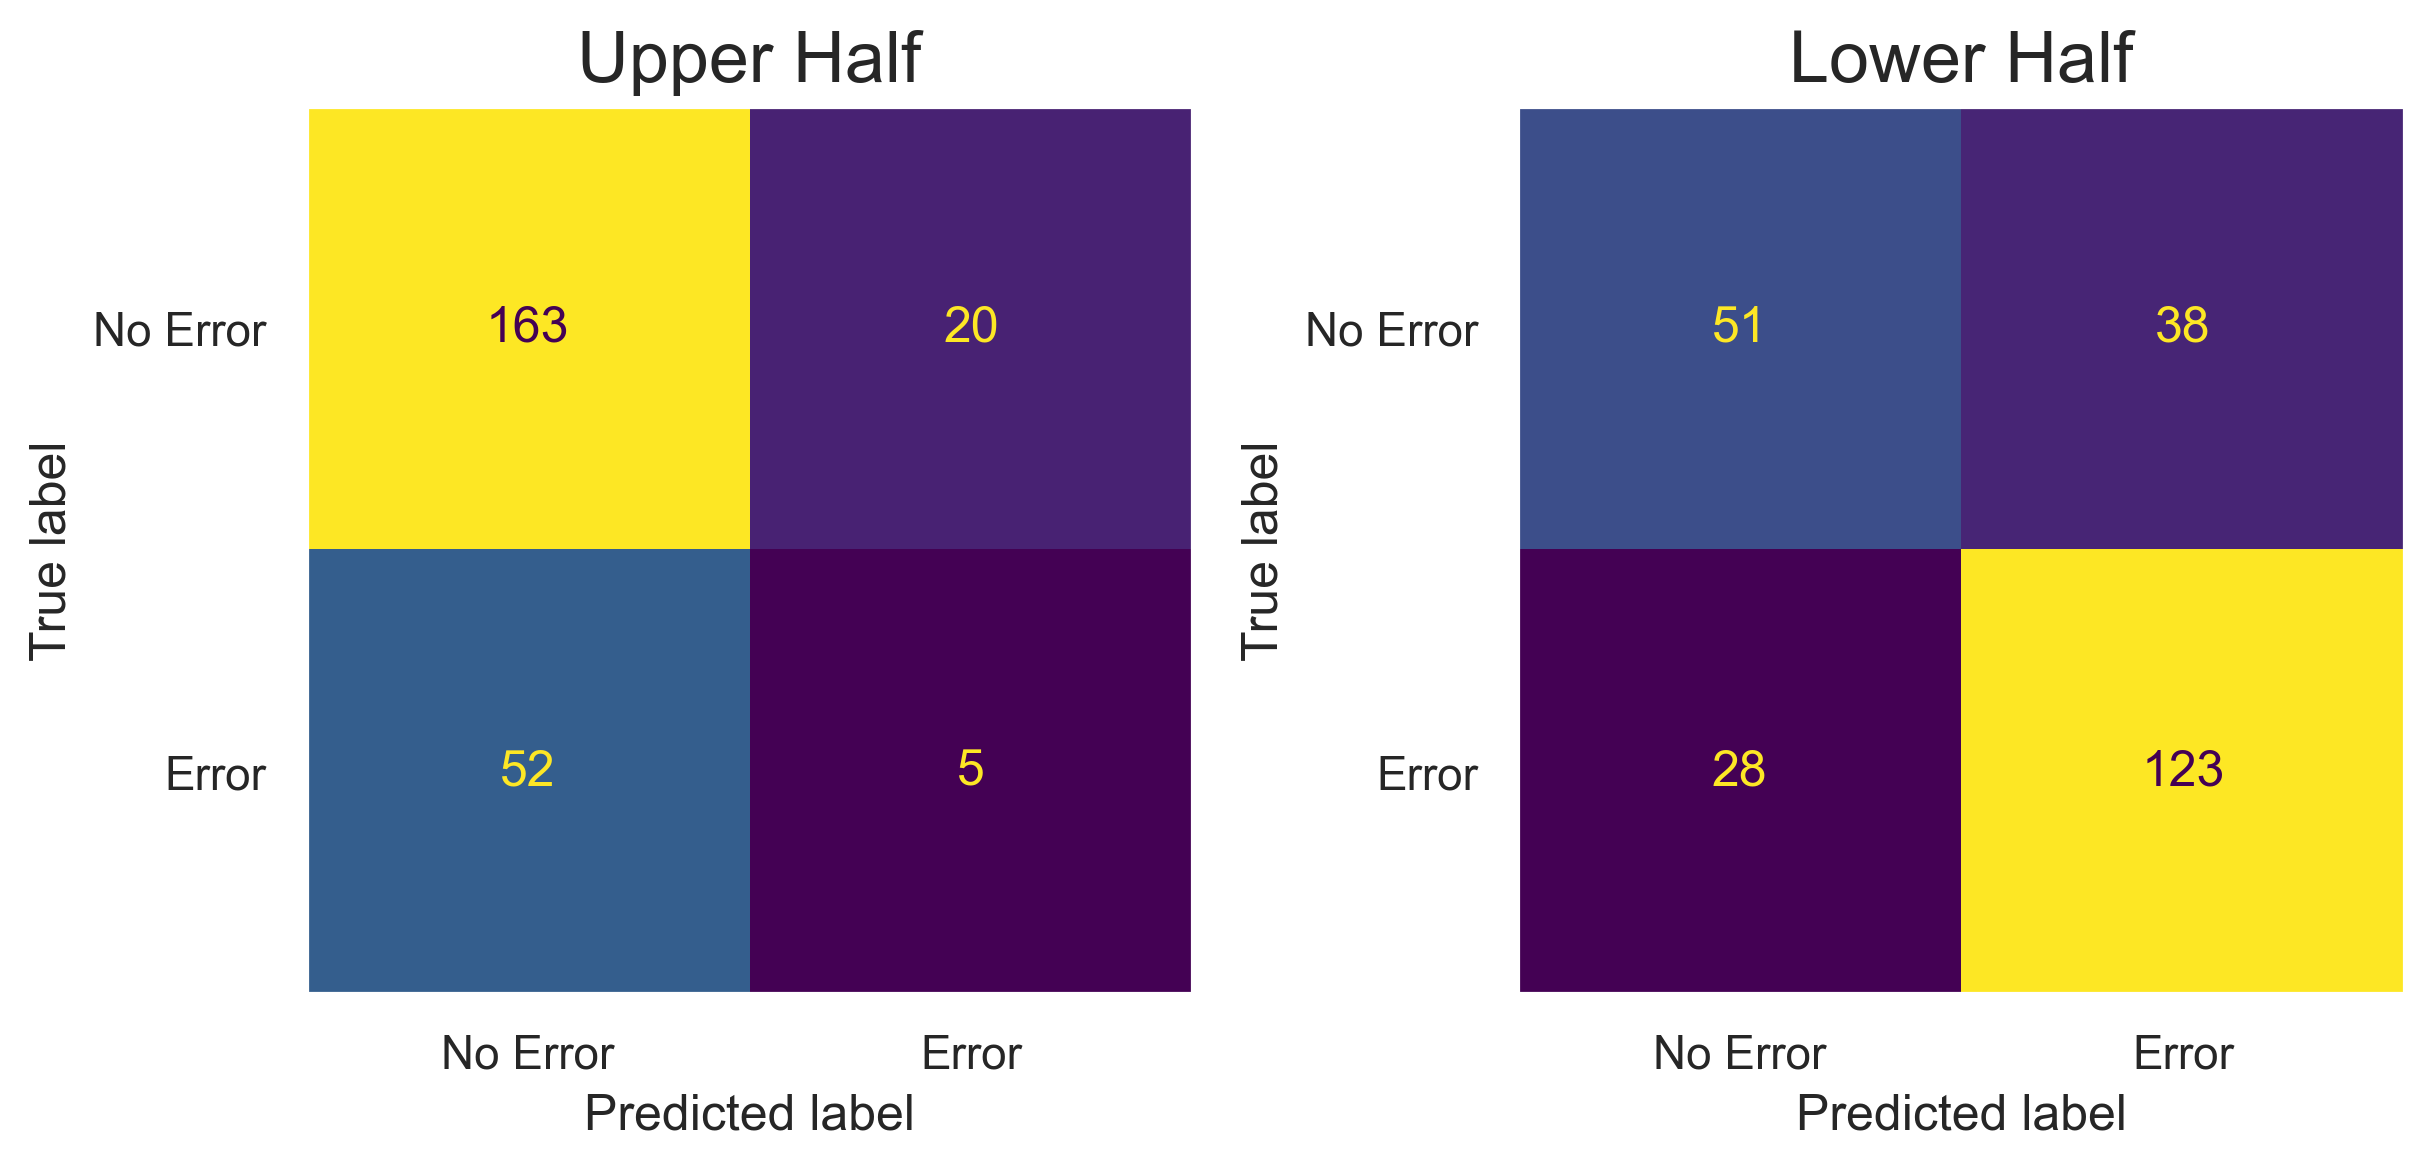
\includegraphics[width=.8\linewidth]{figures/Results/v2/confusion/body_halves_half.png}
  \caption[Confusion matrix of FESDModelv2 for each Body Half]{The confusion matrix of the upper and lower body for FESDModelv2 for the body half problem set.}
  \label{fig:conf_v2_hb_ul}
\end{figure}

\FloatBarrier